\documentclass[a4paper,12pt]{report}
\usepackage[pdftex]{graphicx}
\DeclareGraphicsExtensions{.pdf}
\usepackage{amsmath}
\usepackage{amssymb}

% Title Page
\title{Implementation of ELF in Abinit within the norm-conserving approach}
\author{Aur\'{e}lien Lherbier}


\begin{document}
\maketitle

\begin{abstract}
The aim of this report is first to review some basics of plane waves implementation for electronic structure calculations and more especially plane waves implementation in the Abinit code, and then go to the implementation of the kinetic energy density which is for example required in meta-GGA formalism, but also required for electron function localization (ELF).
\end{abstract}

\chapter{Wavefunction in plane waves representation and symmetries}
\label{chapter1}

\section{Plane waves representation}
\label{section1_1}

In periodic systems, we can express wavefunction ($\psi$) in terms of Bloch wavefunction as

\begin{equation}
\psi_{n\mathbf{k}}(\mathbf{r}) = u_{n\mathbf{k}}(\mathbf{r}) e^{i2\pi \mathbf{k}\cdotp\mathbf{r}}
\end{equation}

where each Bloch wavefunction is characterized by the number of the band $n$\footnote{Here the use band labelling implicitely means that we work only in the 1rst Brillouin zone (see Fig.(\ref{figband_1rstBZ}))} and the wavevector $\mathbf{k}$. The term $u_{n\mathbf{k}}$ gives to the Bloch wavefunction the periodicity of the system

\begin{equation}
u_{n\mathbf{k}}(\mathbf{r}+\mathbf{R}) = u_{n\mathbf{k}}(\mathbf{r})
\end{equation}

where $\mathbf{R}$ is any linear combinations of the real space lattice vectors $\mathbf{R}_{latt}$. Hence we have for the wavefunction
\begin{equation}
\psi_{n\mathbf{k}}(\mathbf{r}+\mathbf{R}) = \psi_{n\mathbf{k}}(\mathbf{r})e^{i2\pi\mathbf{k}\cdotp\mathbf{R}} \label{wf_r+R}
\end{equation}

The term $u_{n\mathbf{k}}$ (and thus also the wavefunction) can be represented in term of plane waves as

\begin{eqnarray}
u_{n\mathbf{k}}(\mathbf{r}) &=& \sum_{\mathbf{G_{\mathbf{k}}}} c_{n\mathbf{k}}(\mathbf{G}_{\mathbf{k}}) e^{i2\pi \mathbf{G}_{\mathbf{k}}\cdotp\mathbf{r}} \\
\psi_{n\mathbf{k}}(\mathbf{r}) &=& \sum_{\mathbf{G_{\mathbf{k}}}} c_{n\mathbf{k}}(\mathbf{G}_{\mathbf{k}}) e^{i2\pi \left(  \mathbf{k} +\mathbf{G}_{\mathbf{k}}\right) \cdotp\mathbf{r}}
\end{eqnarray}

where $e^{i2\pi\mathbf{G}_{\mathbf{k}}\cdotp\mathbf{r}}$ are the plane waves and $c_{n\mathbf{k}}(\mathbf{G}_{\mathbf{k}})$ are their corresponding weigth and actually nothingelse than the Fourier transform components of $u_{n\mathbf{k}}(\mathbf{r})$. Here $\mathbf{G_{\mathbf{k}}}$ are any linear combinations of the reciprocal lattice vectors $\mathbf{G}_{latt}$\footnote{We remind that $\mathbf{G}_{latt}$ is obtained with $\mathbf{G}_{latt,i}\cdotp\mathbf{R}_{latt,j} = \delta_{ij}$. In many textbook you can find $\mathbf{G}_{latt,i}\cdotp\mathbf{R}_{latt,j} = 2\pi \delta_{ij}$ but then you have to define Bloch wavefunction as $\psi_{n\mathbf{k}}(\mathbf{r}) = u_{n\mathbf{k}}(\mathbf{r}) e^{i\mathbf{k}\cdotp\mathbf{r}}$. Both convention are possible it is up to you, here we use the one of Abinit.}. Other theoretical considerations  for Abinit code can be find in \cite{doc1WF_gonze}.\\
In the previous equation we notice the index $\mathbf{k}$ on $\mathbf{G_{\mathbf{k}}}$ which comes from the fact that in practice, to avoid an infinite sum over $\mathbf{G}$ vectors, we limit us (for each $\mathbf{k}$) to a finite number of $\mathbf{G}$ vectors defined by the cut-off energy $E_{kin-cut}$. Therefore $\mathbf{G}_{\mathbf{k}}$ is such that

\begin{equation}
\frac{(2\pi)^2 \vert \mathbf{G}_{\mathbf{k}}+\mathbf{k} \vert^2}{2} < E_{kin-cut} \label{Ecutsphere}
\end{equation}

According to this definition, the number of $\mathbf{G}$ vectors (i.e. number of plane waves) \textit{can} be different for each $\mathbf{k}$ (Fig. \ref{sphere_Gk}), that's why we use an index on $\mathbf{G}$.

\begin{figure}[!h]
\centering
\begin{minipage}[c]{1.0\textwidth}
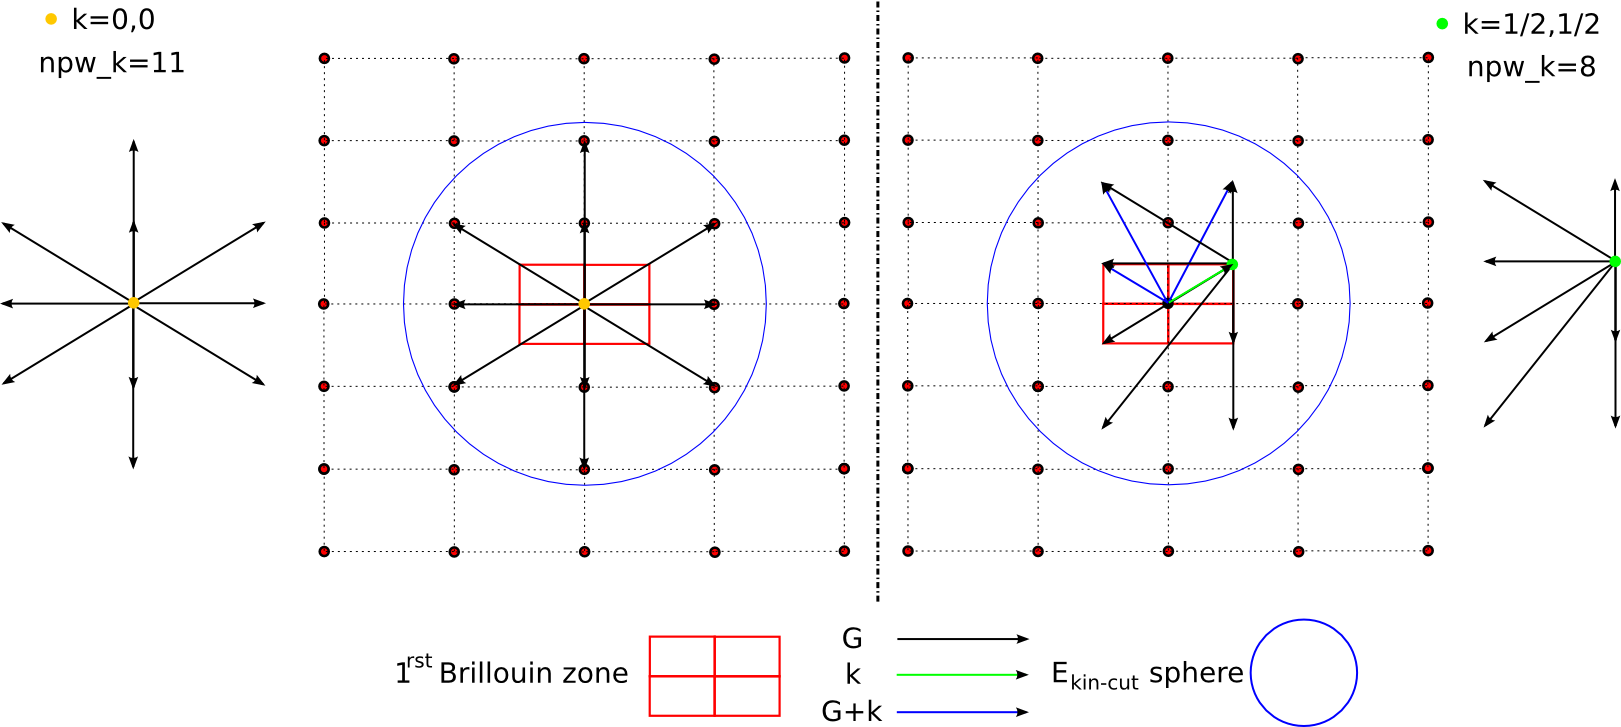
\includegraphics[width = \textwidth]{sphere_Gk}
\end{minipage}
\vspace{0.12\textwidth}
\begin{minipage}[c]{0.9\textwidth}
\caption{\small Schematic view of reciprocal space with $1^{\text{rst}}$ Brillouin zone and associated reciprocal lattice vectors ($\mathbf{G}$) for a simple $2D$ rectangular unit cell. The set of allowed $\mathbf{G}_{\mathbf{k}}$ defined by Eq.(\ref{Ecutsphere}) is represented by a star for two different $\mathbf{k}$ vectors ($\mathbf{k}=0$: left panel, $\mathbf{k}=1/2(\mathbf{G}_{latt,1}+\mathbf{G}_{latt,2})$: right panel). The number of plane waves for each $\mathbf{k}$ (npw\_k) can be different. Note that we count the vector $\mathbf{G}_{\mathbf{k}} = 0$.}
\vspace*{1.0ex}
\label{sphere_Gk}
\end{minipage}
\end{figure}

Hence, rigourously, we should write explicitely for the wavefunction

\begin{equation}
\psi_{n\mathbf{k}}(\mathbf{r}) = \sum_{\mathbf{G_{\mathbf{k}}}}^{\text{npw\_k}} c_{n\mathbf{k}}(\mathbf{G}_{\mathbf{k}}) e^{i2\pi \left(  \mathbf{k} +\mathbf{G}_{\mathbf{k}}\right) \cdotp\mathbf{r}}
\end{equation}

Finally we have a last relation for the wavefunction which is related the fact that we work only in the $1^{\text{rst}}$ Brillouin zone (Fig.(\ref{figband_1rstBZ})).

\begin{eqnarray}
\psi_{n(\mathbf{k}+\mathbf{G})}(\mathbf{r}) &=& \psi_{n\mathbf{k}}(\mathbf{r}) \nonumber \\
\text{and thus,}\quad u_{n(\mathbf{k}+\mathbf{G})}(\mathbf{r}) &=& u_{n\mathbf{k}}(\mathbf{r}) e^{i2\pi \mathbf{G}\cdotp\mathbf{r}} \nonumber
\end{eqnarray}

But we have to precise that when we want to write equatility between two wavefunctions, we should always consider that all linear combinations are also possible. So we introduce the notation $\stackrel{L.C.}{=}$ when this is the case\footnote{Choosing strictly the equality is like doing a choice of gauge.}.

\begin{eqnarray}
\psi_{n(\mathbf{k}+\mathbf{G})}(\mathbf{r}) &\stackrel{L.C.}{=}& \psi_{n\mathbf{k}}(\mathbf{r}) \\
u_{n(\mathbf{k}+\mathbf{G})}(\mathbf{r}) &\stackrel{L.C.}{=}& u_{n\mathbf{k}}(\mathbf{r}) e^{i2\pi \mathbf{G}\cdotp\mathbf{r}}
\end{eqnarray}

\begin{figure}[!h]
\centering
\begin{minipage}[c]{0.69\textwidth}
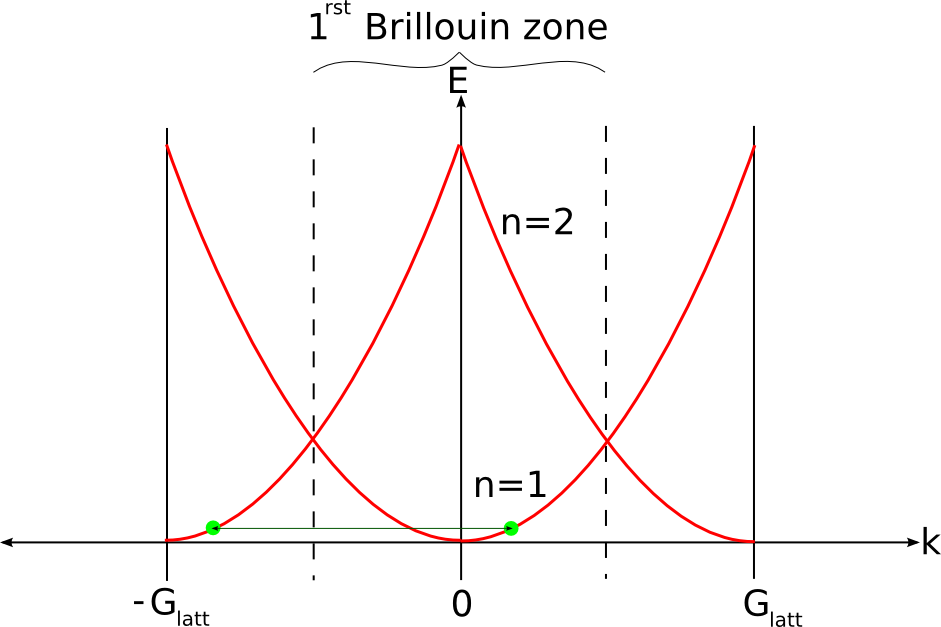
\includegraphics[width = \textwidth]{1rstBZ_free_electron}
\end{minipage}
\vspace{0.05\textwidth}
\begin{minipage}[c]{1.0\textwidth}
\caption{\small Band structure ($E(\mathbf{k})$) for the $1D$ free electron gaz showing the periodicity with respect to reciprocal lattice vectors $\mathbf{G}_{latt}$ which leads to define the $1^{\text{rst}}$ Brillouin zone and the labelling of band ($n$). Working only with $1^{\text{rst}}$ Brillouin zone means that $\psi_{n\mathbf{k}} (\mathbf{r})$ and $\psi_{n(\mathbf{k}+\mathbf{G})}(\mathbf{r})$ gives the same energy $E_{n\mathbf{k}}$.}
\label{figband_1rstBZ}
\end{minipage}
\end{figure}


\section{Symmetries}
\label{section1_2}

In the case of \textit{ab initio} code we are often limited by memory and computational cost, hence we try to reduce the calculation to its minimal cost. That is why we have to take benifit of the symmetries of the problem\footnote{such as time reversal symmetry} and of the system (i.e. the eventual symmetries of the unit cell).\\
In real space we can define the symmetries by a set of symmetry operators $S_{t}$\footnote{The whole set of symmetry operators is called a \textit{space group}.}\cite{burns_glazer_90}. These operators act on real space vectors as

\begin{equation}
S_{t}(\mathbf{r}) = \mathbf{r}'
\end{equation}

Where by example, $\mathbf{r}$ is vector pointing on an atom and $\mathbf{r}'$ is the vector pointing on the symmetric atom. The different possible symmetry operations are identity, inversion, (mirror-)reflections, rotations, rotation-inversions\footnote{which combines a rotation plus an inversion operation. Why define a such combined operation? Because actually, even if a crystal has not the rotation and the inversion symmetry (individually) it can have the rotation-inversion symmetry.}, translations, screw rotations\footnote{which combines a rotation plus a translation operation.} and glide reflections\footnote{which combines a reflection plus a translation operation.}. The first symmetry operations: identity, inversion, reflections, rotations and rotation-inversion; are called symmorphic operations ($S$) and can be described in matrix representation by $3\times3$ matrices $S_{\alpha\beta}$ as

\begin{equation}
\mathbf{r}'= S(\mathbf{r}) \qquad \Rightarrow \qquad r'_{\alpha} = \sum_{\beta} S_{\alpha\beta} \,r_{\beta}
\end{equation}

For translation operations and other operations which are combined with translation (screw rotations and glide reflections) we need a translation vector $\mathbf{t}$. For simple translation we have

\begin{equation}
\mathbf{r}'= \mathbf{r}+\mathbf{t} \qquad \Rightarrow \qquad r'_{\alpha} = r_{\alpha} + t_{\alpha}
\end{equation}

For screw rotations and glide reflections we have

\begin{equation}
\mathbf{r}'= S(\mathbf{r})+\mathbf{t} \qquad \Rightarrow \qquad r'_{\alpha} = \sum_{\beta} S_{\alpha\beta}\, r_{\beta} + t_{\alpha}
\end{equation}

For practical reasons it is better to group all symmetry operation types in a single representation, so we use the most general form (the screw rotations and glide reflections form) and we define the generalized operator $S_{\mathbf{t}}$\footnote{The generalized operator $S_{\mathbf{t}}$ is also called a \textit{Seitz operator}.} as

\begin{equation}
\mathbf{r}'= S_{\mathbf{t}}(\mathbf{r}) \qquad \Rightarrow \qquad r'_{\alpha} = \sum_{\beta} S_{\alpha\beta} \,r_{\beta} + t_{\alpha} \label{eqStdef}
\end{equation}

where in the case of symmorphic operations the vector $\mathbf{t}$ is $\overrightarrow{0}$; and in the case of pure translation operations the matrix $S_{\alpha\beta}$ is the identity matrix.\\
When applying these symmetry operators to the wavefunction we get

\begin{equation}
\psi_{n\mathbf{k}}' \stackrel{L.C.}{=} S_{\mathbf{t}} \left( \psi_{n\mathbf{k}}\right)
\end{equation}

where here $S_{\mathbf{t}}$ is acting no more on real space but on the wavefunction space. Consider that the wavefunction is a vector of wavefunction space, $S_{\mathbf{t}}$ transforms this wavefunction vector into another wavefunction vector. Our goal is to know what is this symmetrized wavefunction compared to the starting wavefunction. Since the wavefunction is a function of real space we can have the relation

\begin{equation}
\left(S_{\mathbf{t}} \left( \psi_{n\mathbf{k}}\right) \right)(\mathbf{r}) \stackrel{L.C.}{=} \psi_{n\mathbf{k}}' (\mathbf{r}) \stackrel{L.C.}{=} \psi_{n\mathbf{k}}(S_{\mathbf{t}}^{-1}\left( \mathbf{r}\right) ) \label{eqs-1}
\end{equation}

Notice that this not the same operation as

\begin{equation}
S_{\mathbf{t}} \left( \psi_{n\mathbf{k}}(\mathbf{r})\right) \stackrel{L.C.}{=} \psi_{n\mathbf{k}}' (S_{\mathbf{t}}(\mathbf{r})) \stackrel{L.C.}{=} \psi_{n\mathbf{k}}( \mathbf{r})
\end{equation}

In Eq.(\ref{eqs-1}) we apply the inverse of the symmetry operator ($S_{\mathbf{t}}^{-1}$) to the real space vector $\mathbf{r}$ which is defined by

\begin{equation}
\mathbf{r}' = S_{\mathbf{t}}^{-1}\left( \mathbf{r}\right)  \qquad \Rightarrow  \qquad r_{\alpha}' = \sum_{\beta} S_{\alpha \beta}^{-1}\left( r_{\beta} - t_{\beta}\right)
\end{equation}

Now let's have a look at the symmetry operator applied to the wavefunction taken at $\mathbf{r}+\mathbf{R}$.

\begin{equation}
\left( S_{\mathbf{t}} \left( \psi_{n\mathbf{k}}\right) \right) (\mathbf{r}+\mathbf{R}) \stackrel{L.C.}{=} \psi_{n\mathbf{k}}'(\mathbf{r}+\mathbf{R}) \stackrel{L.C.}{=} \psi_{n\mathbf{k}}(S_{\mathbf{t}}^{-1}\left( \mathbf{r}+\mathbf{R}\right) ) \label{eqA}
\end{equation}

where $S_{\mathbf{t}}^{-1}\left( \mathbf{r}+\mathbf{R}\right)$ is

\begin{eqnarray}
\mathbf{r}'' = S_{\mathbf{t}}^{-1}\left( \mathbf{r}+\mathbf{R}\right) \qquad &\Rightarrow&  \qquad r_{\alpha}'' = \sum_{\beta} S_{\alpha \beta}^{-1}\left( r_{\beta} + R_{\beta} - t_{\beta}\right) \nonumber \\
&& \qquad r_{\alpha}'' = \sum_{\beta} S_{\alpha \beta}^{-1}\left( r_{\beta} - t_{\beta}\right) + \sum_{\beta} S_{\alpha \beta}^{-1}R_{\beta} \nonumber \\
&& \qquad r_{\alpha}'' = r_{\alpha}' + \tilde{R}_{\alpha} \nonumber\\
\mathbf{r}'' = \mathbf{r}' + \tilde{\mathbf{R}} \qquad \qquad \quad&& \nonumber\\
\mathbf{r}'' =  S_{\mathbf{t}}^{-1}\left( \mathbf{r}\right) +  S^{-1}\left(\mathbf{R}\right)  &&
\end{eqnarray}

Hence, in virtue of Eq.(\ref{wf_r+R}) and previous result, we have

\begin{eqnarray}
\left( S_{\mathbf{t}} \left( \psi_{n\mathbf{k}}\right) \right) (\mathbf{r}+\mathbf{R}) \stackrel{L.C.}{=} \psi_{n\mathbf{k}}(\mathbf{r}'') &\stackrel{L.C.}{=}& \psi_{n\mathbf{k}}(S_{\mathbf{t}}^{-1}\left( \mathbf{r}\right) + S^{-1}\left(\mathbf{R}\right)) \nonumber \\
&\stackrel{L.C.}{=}& \psi_{n\mathbf{k}}(S_{\mathbf{t}}^{-1}\left( \mathbf{r}\right)) e^{i2\pi\mathbf{k}\cdotp\left(S^{-1}\left(\mathbf{R}\right)\right) }
\end{eqnarray}

Now the final step is to rewrite the phase factor $e^{i2\pi\mathbf{k}\cdotp\left(S^{-1}\left(\mathbf{R}\right)\right)}$ in order to transfer the $S^{-1}$ operator,which is acting on $\mathbf{R}$ (real space), to $\mathbf{k}$ (reciprocal space). For that we use the transposed of $S^{-1}$

\begin{eqnarray}
e^{i2\pi\mathbf{k}\cdotp\left(S^{-1}\left(\mathbf{R}\right)\right) } &=& e^{i2\pi \sum_{\alpha}k_{\alpha} \left(\sum_{\beta}S^{-1}_{\alpha\beta} R_{\beta}\right) } \nonumber \\
e^{i2\pi\mathbf{k}\cdotp\left(S^{-1}\left(\mathbf{R}\right)\right) } &=& e^{i2\pi \sum_{\alpha\beta}k_{\alpha} S^{-1}_{\alpha\beta} R_{\beta} } \nonumber \\
e^{i2\pi\mathbf{k}\cdotp\left(S^{-1}\left(\mathbf{R}\right)\right) } &=& e^{i2\pi \sum_{\beta} \left(\sum_{\alpha} k_{\alpha} S^{-1,\mathtt{t}}_{\beta\alpha}\right) R_{\beta} } \nonumber \\
e^{i2\pi\mathbf{k}\cdotp\left(S^{-1}\left(\mathbf{R}\right)\right) } &=& e^{i2\pi\left(S^{-1,\mathtt{t}}\left(\mathbf{k}\right)\right)\cdotp\mathbf{R} }
\end{eqnarray}

Let's call $\mathbf{k}'$ the new vector such as

\begin{equation}
\mathbf{k}' = S^{-1,\mathtt{t}}\left( \mathbf{k}\right)  \qquad \Rightarrow  \qquad k_{\beta}' = \sum_{\alpha} S_{\beta\alpha}^{-1,\mathtt{t}} k_{\alpha}
\end{equation}

Notice that to obtain $\mathbf{k}'$ from $\mathbf{k}$ we use the symmetry operator without the translation operation, i.e. we have used only the symmorphic part of the symmetry operation.
Finally we have

\begin{eqnarray}
\left( S_{\mathbf{t}} \left( \psi_{n\mathbf{k}}\right) \right) (\mathbf{r}+\mathbf{R}) \stackrel{L.C.}{=}  \psi_{n\mathbf{k}}'(\mathbf{r}+\mathbf{R}) &\stackrel{L.C.}{=}& \psi_{n\mathbf{k}}(S_{\mathbf{t}}^{-1}\left( \mathbf{r}\right)) e^{i2\pi\mathbf{k}'\cdotp\mathbf{R}} \nonumber\\
\stackrel{L.C.}{=} \psi_{n\mathbf{k}}'(\mathbf{r}+\mathbf{R}) &\stackrel{L.C.}{=}& \psi_{n\mathbf{k}}'(\mathbf{r}) e^{i2\pi\mathbf{k}'\cdotp\mathbf{R}}
\end{eqnarray}

which actually means that the symmetrized wavefunction $\psi_{n\mathbf{k}}'$ is the Bloch wavefunction at $\mathbf{k}'$ (see Eq.(\ref{wf_r+R})), thus

\begin{equation}
\left( S_{\mathbf{t}} \left( \psi_{n\mathbf{k}}\right) \right) (\mathbf{r}) \stackrel{L.C.}{=} \psi_{n\mathbf{k}}'(\mathbf{r}) \stackrel{L.C.}{=} \psi_{n\mathbf{k}'}(\mathbf{r}) \label{symrel_psikkprime}
\end{equation}

In Abinit code we store only the weigth of each plane wave ($c_{n\mathbf{k}}(\mathbf{G_{\mathbf{k}}})$) so we are more interested to find relation between $c_{n\mathbf{k}}(\mathbf{G_{\mathbf{k}}})$

\begin{eqnarray}
\left( S_{\mathbf{t}} \left( \psi_{n\mathbf{k}}\right) \right) (\mathbf{r}) &\stackrel{L.C.}{=}&  \psi_{n\mathbf{k}'}(\mathbf{r}) \nonumber \\
\psi_{n\mathbf{k}}(S_{\mathbf{t}}^{-1} (\mathbf{r})) &\stackrel{L.C.}{=}&  \psi_{n\mathbf{k}'}(\mathbf{r}) \nonumber \\
\sum_{\mathbf{G_{\mathbf{k}}}}^{\text{npw\_k}} c_{n\mathbf{k}}(\mathbf{G}_{\mathbf{k}}) e^{i2\pi \left(  \mathbf{k} +\mathbf{G}_{\mathbf{k}}\right)\cdotp(S_{\mathbf{t}}^{-1} (\mathbf{r}))} &\stackrel{L.C.}{=}& \sum_{\mathbf{G_{\mathbf{k}'}}}^{\text{npw\_k'}} c_{n\mathbf{k}'}(\mathbf{G}_{\mathbf{k}'}) e^{i2\pi \left(  \mathbf{k}' +\mathbf{G}_{\mathbf{k}'}\right)\cdotp\mathbf{r}}
\end{eqnarray}

At this stage we have to specify two things:\\
First we can easily see that npw\_k = npw\_k' because $\vert\mathbf{k}\vert =\vert\mathbf{k}'\vert$ (see Eq.(\ref{Ecutsphere}) and Fig.(\ref{sphere_Gk}) for instance). Indeed $\mathbf{k}'$ is obtained from symmorphic operation ($S^{-1,\mathtt{t}}$) applied to $\mathbf{k}$ (that is all symmetry operation but the ones with translations, which leads to preserve the modulus of the vector). This is important to get a one to one correspondance at the end.\\
Secondly, what is $\mathbf{G}_{\mathbf{k}'}$ compared to $\mathbf{G}_{\mathbf{k}}$. Actually this is just (see Fig.(\ref{sym_Gk}))

\begin{equation}
\mathbf{G}_{\mathbf{k}'} = \mathbf{G}_{\mathbf{k}}' = S^{-1,{\mathtt{t}}}\left( \mathbf{G}_{\mathbf{k}}\right)  \qquad \Rightarrow  \qquad G_{\mathbf{k}',\beta} =G_{\mathbf{k},\beta}' = \sum_{\alpha} S_{\beta\alpha}^{-1,{\mathtt{t}}} G_{\mathbf{k},\alpha}
\end{equation}

\begin{figure}[!ht]
\centering
\begin{minipage}[c]{1.0\textwidth}
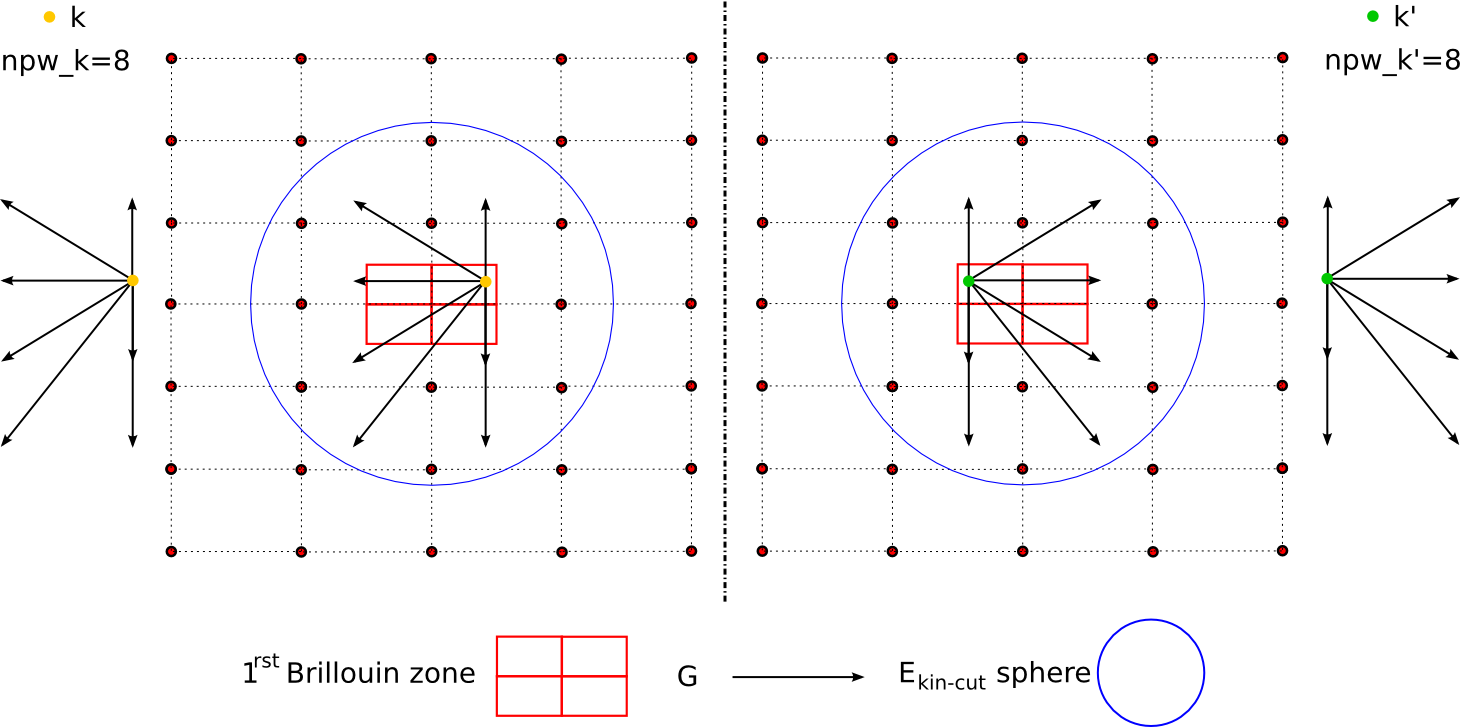
\includegraphics[width = \textwidth]{sym_Gk}
\end{minipage}
\vspace{0.27\textwidth}
\begin{minipage}[c]{0.8\textwidth}
\caption{\small Schematic view of reciprocal space with $1^{\text{rst}}$ Brillouin zone and associated reciprocal lattice vectors ($\mathbf{G}$) for a simple $2D$ rectangular unit cell. The set of allowed $\mathbf{G}_{\mathbf{k}}$ defined by Eq.(\ref{Ecutsphere}) is represented by a star for two symmetric $\mathbf{k}$ vectors ($\mathbf{k}$ :left panel, $\mathbf{k}'$: right panel). The number of plane waves for symmetric $\mathbf{k}$ (npw\_k) is the same, and $\mathbf{k}$-associated plane waves are symmetric to $\mathbf{k}'$-associated plane waves.}
\vspace*{1.0ex}
\label{sym_Gk}
\end{minipage}
\end{figure}

so we have

\begin{equation}
\sum_{\mathbf{G_{\mathbf{k}}}}^{\text{npw\_k}} c_{n\mathbf{k}}(\mathbf{G}_{\mathbf{k}}) e^{i2\pi \sum_{\alpha\beta} \left( k_{\alpha} + G_{\mathbf{k},\alpha}\right) S_{\alpha\beta}^{-1} \left(r_{\beta}-t_{\beta}\right)} = \sum_{\mathbf{G_{\mathbf{k}}'}}^{\text{npw\_k'}} c_{n\mathbf{k}'}(\mathbf{G}_{\mathbf{k}}') e^{i2\pi \sum_{\alpha\beta} \left(k_{\alpha} + G_{\mathbf{k},\alpha}\right)S_{\beta\alpha}^{-1,\mathtt{t}} r_{\beta}} \nonumber
\end{equation}

which yields to

\begin{eqnarray}
c_{n\mathbf{k}}(\mathbf{G}_{\mathbf{k}}) e^{-i2\pi \sum_{\alpha\beta} \left( k_{\alpha} + G_{\mathbf{k},\alpha}\right) S_{\alpha\beta}^{-1} t_{\beta}} &=& c_{n\mathbf{k}'}(\mathbf{G}_{\mathbf{k}}') \nonumber \\
c_{n\mathbf{k}}(\mathbf{G}_{\mathbf{k}}) e^{-i2\pi \left( \mathbf{k}' + \mathbf{G}_{\mathbf{k}}'\right)\cdotp \mathbf{t}} &=& c_{n\mathbf{k}'}(\mathbf{G}_{\mathbf{k}}') \nonumber \\
c_{n\mathbf{k}}(\mathbf{G}_{\mathbf{k}}) &=& c_{n\mathbf{k}'}(\mathbf{G}_{\mathbf{k}}') e^{+i2\pi \left( \mathbf{k}' + \mathbf{G}_{\mathbf{k}}'\right)\cdotp \mathbf{t}}
\end{eqnarray}

or in a equivalent manner\footnote{Indeed we can interchange $\mathbf{k}'$ and $\mathbf{G}_{\mathbf{k}}'$ with $\mathbf{k}$ and $\mathbf{G}_{\mathbf{k}}$ by considering the inverse symmetry operation.}

\begin{equation}
c_{n\mathbf{k}'}(\mathbf{G}_{\mathbf{k}}') = c_{n\mathbf{k}}(\mathbf{G}_{\mathbf{k}}) e^{+i2\pi \left( \mathbf{k} + \mathbf{G}_{\mathbf{k}}\right)\cdotp \mathbf{t}} \label{cnkG_cnk'G'_rel}
\end{equation}

Remember now how we have defined the generalized symmetry operator $S_{\mathbf{t}}$ (Eq.\ref{eqStdef}). For the previous result, it means that for all symmorphic symmetry operations (i.e. when $\mathbf{t}=\overrightarrow{0}$) we have the simple relation

\begin{equation}
c_{n\mathbf{k}'}(\mathbf{G}_{\mathbf{k}}') = c_{n\mathbf{k}}(\mathbf{G}_{\mathbf{k}})
\end{equation}

Notably for the inversion symmetry operation we have

\begin{equation}
c_{n(\mathbf{k}'=-\mathbf{k})}((\mathbf{G}_{\mathbf{k}}'=-\mathbf{G}_{\mathbf{k}})) = c_{n\mathbf{k}}(\mathbf{G}_{\mathbf{k}})
\end{equation}

and for the wavefunction (using Eq.(\ref{symrel_psikkprime}))

\begin{equation}
\psi_{n\mathbf{k}}(-\mathbf{r}) \stackrel{L.C.}{=} \psi_{n(-\mathbf{k})}(\mathbf{r})
\end{equation}

To finish this section on the use of symmetries, we can add another type of symmetry which has not yet been taken into account because this is not a space group symmetry but a symmetry of the problem; that is the time reversal symmetry (for non-magnetic case) which is

\begin{equation}
\psi_{n\mathbf{k}}(\mathbf{r}) \stackrel{L.C.}{=} \psi_{n(-\mathbf{k})}^{*}(\mathbf{r})
\end{equation}

which for $c_{n\mathbf{k}}(\mathbf{G}_{\mathbf{k}})$ gives the relation
\begin{equation}
c_{n\mathbf{k}}(\mathbf{G}_{\mathbf{k}}) = c_{n(-\mathbf{k})}^{*}(-\mathbf{G}_{\mathbf{k}})
\end{equation}


\chapter{Electronic density and kinetic energy density}
\label{chapter2}

We are going to look now at two quantities which are electronic density and kinetic energy density. We treat them in the same chapter because they have quite similar forms\footnote{their implementations in ABINIT are thus grouped in a single routine (\textit{mkrho}).}.

\section{Electronic density}
\label{section2_1}

The electronic density ($n(\mathbf{r})$) is given by

\begin{equation}
n(\mathbf{r}) = \sum_{\mathbf{k}} \sum_n f(E_{n\mathbf{k}}) \vert \psi_{n\mathbf{k}}(\mathbf{r}) \vert^2
\end{equation}

where $f(E)$ is the Fermi-Dirac distribution.\\
Let's work at zero temperature and reduce the sum to a sum over the states below and up to the Fermi level ($E_f$)\footnote{the Fermi-Dirac distribution becomes $f(E)=1$ when $E\leq E_f$ and $f(E)=0$ otherwise.}.

\begin{equation}
n(\mathbf{r}) = \sum_{\mathbf{k}} \sum_n \vert \psi_{n\mathbf{k}}(\mathbf{r}) \vert^2
\end{equation}

Consider also that the system might have some symmetries and from what we have seen in the previous chapter it is thus possible to reduce again the sum to a sum over an irreducible set of $\mathbf{k}$ vectors. It corresponds to what we call the irreducible Brillouin zone ($IBZ$). See figure (Fig.(\ref{fig_IBZ})) for an example.\\

\begin{figure}[!t]
\centering
\begin{minipage}[c]{0.45\textwidth}
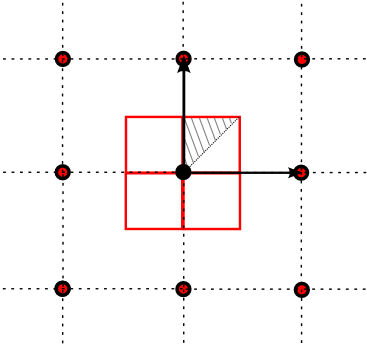
\includegraphics[width = \textwidth]{IBZ}
\end{minipage}
\vspace{0.1\textwidth}
\begin{minipage}[c]{0.8\textwidth}
\caption{\small Schematic view of reciprocal space with $1^{\text{rst}}$ Brillouin zone and associated reciprocal lattice vectors ($\mathbf{G}$) for a simple $2D$ cubic unit cell. The irreducible Brillouin zone ($IBZ$) is represented by the hatched triangle.}
\vspace*{0.5ex}
\label{fig_IBZ}
\end{minipage}
\end{figure}

Hence the electronic density can be cutted in symmetric part and thus is now written as a sum over symmetry operators applied to electronic density part defined in the $IBZ$,

\begin{equation}
n(\mathbf{r}) = \sum_{S_{\mathbf{t}}} \left( S_{\mathbf{t}}\, n^{IBZ} \right) (\mathbf{r}) = \sum_{S_{\mathbf{t}}} n^{IBZ} \left(S_{\mathbf{t}}^{-1}(\mathbf{r})\right) \label{eqnIBZr}
\end{equation}

where $n^{IBZ}$ is the electronic density part defined in the $IBZ$,

\begin{equation}
n^{IBZ}(\mathbf{r}) = \sum_{\mathbf{k} \in IBZ} \sum_n \vert \psi_{n\mathbf{k}}(\mathbf{r}) \vert^2 = \sum_{\mathbf{k} \in IBZ} \sum_n n^{IBZ}_{n\mathbf{k}}(\mathbf{r})
\end{equation}

For the total electronic density, we have

\begin{eqnarray}
n(\mathbf{r}) &=& \sum_{S_{\mathbf{t}}} \left( S_{\mathbf{t}}\, \sum_{\mathbf{k} \in IBZ} \sum_n n^{IBZ}_{n\mathbf{k}} \right) (\mathbf{r}) \label{eqnIBZr2}\\
n(\mathbf{r}) &=& \sum_{S_{\mathbf{t}}} \sum_{\mathbf{k} \in IBZ} \sum_n n^{IBZ}_{n\mathbf{k}} (S_{\mathbf{t}}^{-1} (\mathbf{r})) \nonumber\\
n(\mathbf{r}) &=& \sum_{S_{\mathbf{t}}} \sum_{\mathbf{k} \in IBZ} \sum_n \left( \sum_{\mathbf{G}_{\mathbf{k}}} c_{n\mathbf{k}}^{*}(\mathbf{G}_{\mathbf{k}}) e^{-i2\pi \left( \mathbf{k} + \mathbf{G}_{\mathbf{k}}\right)\cdotp \left( S_{\mathbf{t}}^{-1} (\mathbf{r})\right) } \sum_{\tilde{\mathbf{G}}_{\mathbf{k}}} c_{n\mathbf{k}}(\tilde{\mathbf{G}}_{\mathbf{k}}) e^{i2\pi \left( \mathbf{k} + \tilde{\mathbf{G}}_{\mathbf{k}}\right)\cdotp \left( S_{\mathbf{t}}^{-1} (\mathbf{r})\right) } \right) \nonumber\\
n(\mathbf{r}) &=& \sum_{S_{\mathbf{t}}} \sum_{\mathbf{k} \in IBZ} \sum_n \left( \sum_{\mathbf{G}_{\mathbf{k}}} \sum_{\tilde{\mathbf{G}}_{\mathbf{k}}} c_{n\mathbf{k}}^{*}(\mathbf{G}_{\mathbf{k}}) c_{n\mathbf{k}}(\tilde{\mathbf{G}}_{\mathbf{k}}) e^{i2\pi \left( \tilde{\mathbf{G}}_{\mathbf{k}} -\mathbf{G}_{\mathbf{k}} \right)\cdotp \left( S_{\mathbf{t}}^{-1} (\mathbf{r})\right) } \right)
\end{eqnarray}

We could use this last equation with the double sum over plane waves vectors set ($\mathbf{G}_{\mathbf{k}}$) to compute the electronic density but in practice it is better for numerical cost to make appear a Fourier transform from this last equation and use the performant Fast Fourier Transform (FFT) tools. Indeed we can define a new set of plane waves vectors ($\tilde{\tilde{\mathbf{G}}}_{\mathbf{k}} = \tilde{\mathbf{G}}_{\mathbf{k}} -\mathbf{G}_{\mathbf{k}}$), which will be a larger set of plane waves vectors\footnote{ In Abinit this larger set of plane waves vectors is actually even larger and become $\mathbf{k}$-independent ($\tilde{\tilde{\mathbf{G}}}$). This new larger set of plane waves vectors defines what we call the FFT box.} (see Fig.(\ref{fig_FFTbox})).\\

\begin{figure}[!ht]
\centering
\begin{minipage}[c]{1.0\textwidth}
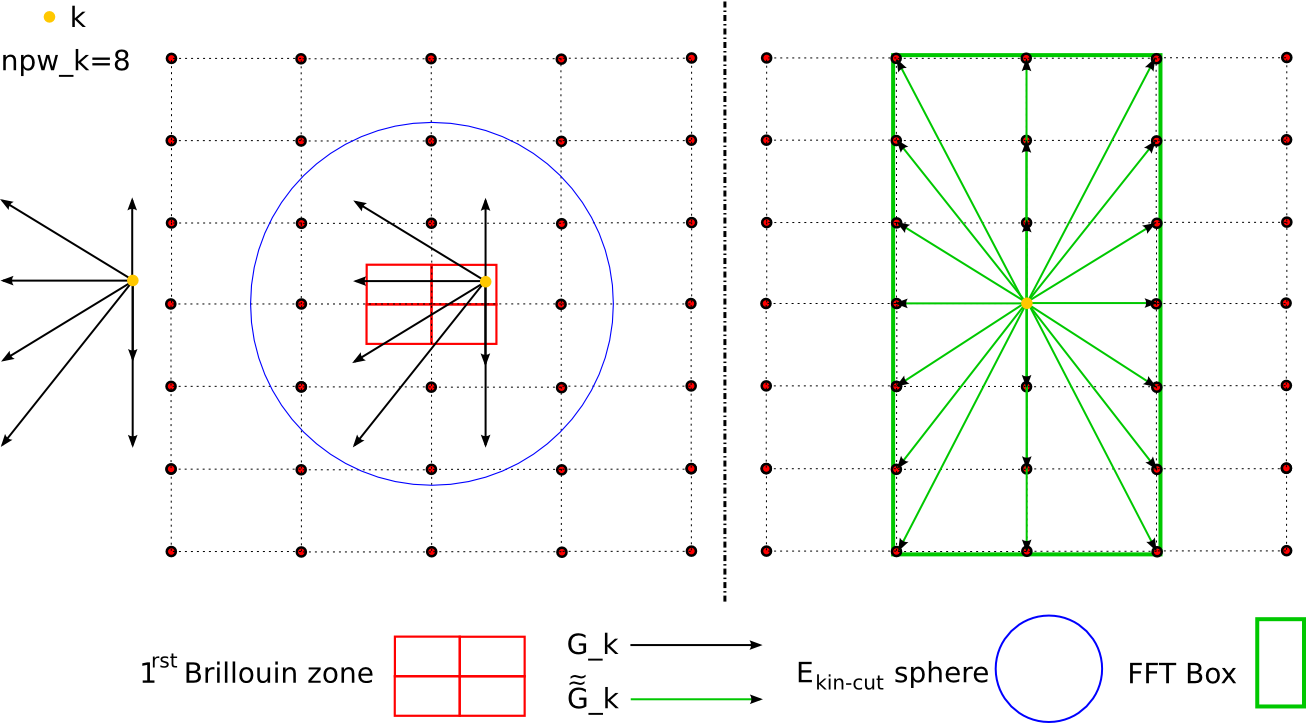
\includegraphics[width = \textwidth]{FFTbox}
\end{minipage}
\vspace{0.27\textwidth}
\begin{minipage}[c]{0.8\textwidth}
\caption{\small Left: Schematic view of reciprocal space with $1^{\text{rst}}$ Brillouin zone and associated reciprocal lattice vectors ($\mathbf{G}$) for a simple $2D$ rectangular unit cell. The set of allowed $\mathbf{G}_{\mathbf{k}}$ defined by Eq.(\ref{Ecutsphere}) is represented by a star for a given $\mathbf{k}$ vector. Right: The corresponding FFT box defined by $\tilde{\tilde{\mathbf{G}}}_{\mathbf{k}} = \tilde{\mathbf{G}}_{\mathbf{k}} -\mathbf{G}_{\mathbf{k}}$.}
\vspace*{1.0ex}
\label{fig_FFTbox}
\end{minipage}
\end{figure}

The electronic density becomes
\begin{eqnarray}
n(\mathbf{r}) &=& \sum_{S_{\mathbf{t}}} \sum_{\mathbf{k} \in IBZ} \sum_n \left( \sum_{\mathbf{G}_{\mathbf{k}}} \sum_{\tilde{\tilde{\mathbf{G}}}_{\mathbf{k}}} c_{n\mathbf{k}}^{*}(\mathbf{G}_{\mathbf{k}}) c_{n\mathbf{k}}(\tilde{\tilde{\mathbf{G}}}_{\mathbf{k}}+\mathbf{G}_{\mathbf{k}}) e^{i2\pi \tilde{\tilde{\mathbf{G}}}_{\mathbf{k}} \cdotp \left( S_{\mathbf{t}}^{-1} (\mathbf{r})\right) } \right) \nonumber \\
n(\mathbf{r}) &=& \sum_{S_{\mathbf{t}}} \sum_{\tilde{\tilde{\mathbf{G}}}_{\mathbf{k}}} \left( \sum_{\mathbf{k} \in IBZ} \sum_n \sum_{\mathbf{G}_{\mathbf{k}}}  c_{n\mathbf{k}}^{*}(\mathbf{G}_{\mathbf{k}}) c_{n\mathbf{k}}(\tilde{\tilde{\mathbf{G}}}_{\mathbf{k}}+\mathbf{G}_{\mathbf{k}})\right) e^{i2\pi \tilde{\tilde{\mathbf{G}}}_{\mathbf{k}} \cdotp \left( S_{\mathbf{t}}^{-1} (\mathbf{r})\right) }  \nonumber \\
n(\mathbf{r}) &=& \sum_{S_{\mathbf{t}}} \sum_{\tilde{\tilde{\mathbf{G}}}_{\mathbf{k}}} \tilde{n}^{IBZ}(\tilde{\tilde{\mathbf{G}}}_{\mathbf{k}})\; e^{i2\pi \tilde{\tilde{\mathbf{G}}}_{\mathbf{k}} \cdotp \left( S_{\mathbf{t}}^{-1} (\mathbf{r})\right) }
\end{eqnarray}

Comparing this last result with Eq.(\ref{eqnIBZr}) we clearly see that $\tilde{n}^{IBZ}(\tilde{\tilde{\mathbf{G}}}_{\mathbf{k}})$ are Fourier transform components of $n^{IBZ}\left(S_{\mathbf{t}}^{-1}(\mathbf{r})\right)$. Moreover you can see that $\tilde{n}^{IBZ}(\tilde{\tilde{\mathbf{G}}}_{\mathbf{k}})$ is independent of the symmetry operators $S$ and then can be computed by FFT with considering whatever symmetry operation we want. In practice we choose off course the identity meaning that we use directly the part of the electronic density computed in the $IBZ$ ($n^{IBZ}(\mathbf{r})$).\\
The idea is now to transfer the sum over symmetry operators which is acting on real space ($S_{\mathbf{t}}^{-1}(\mathbf{r})$) to the reciprocal space\footnote{as we have already done for wavefunction symmetrization in previous chapter}.

\begin{eqnarray}
n(\mathbf{r}) &=& \sum_{\tilde{\tilde{\mathbf{G}}}_{\mathbf{k}}} \sum_{S_{\mathbf{t}}} \tilde{n}^{IBZ}(\tilde{\tilde{\mathbf{G}}}_{\mathbf{k}})\; e^{i2\pi \sum_{\alpha} \tilde{\tilde{G}}_{\mathbf{k},\alpha} \left( \sum_{\beta} S^{-1}_{\alpha\beta} (r_{\beta}-t_{\beta})\right) } \nonumber \\
n(\mathbf{r}) &=& \sum_{\tilde{\tilde{\mathbf{G}}}_{\mathbf{k}}} \sum_{S_{\mathbf{t}}} \tilde{n}^{IBZ}(\tilde{\tilde{\mathbf{G}}}_{\mathbf{k}})\; e^{i2\pi \sum_{\alpha\beta} \tilde{\tilde{G}}_{\mathbf{k},\alpha} S^{-1,{\mathtt{t}}}_{\beta\alpha} (r_{\beta}-t_{\beta}) } \nonumber \\
n(\mathbf{r}) &=& \sum_{\tilde{\tilde{\mathbf{G}}}_{\mathbf{k}}} \sum_{S_{\mathbf{t}}} \tilde{n}^{IBZ}(\tilde{\tilde{\mathbf{G}}}_{\mathbf{k}})\; e^{i2\pi \left( S^{-1,{\mathtt{t}}} (\tilde{\tilde{\mathbf{G}}}_{\mathbf{k}}) \right) \cdot (\mathbf{r}-\mathbf{t}) }
\end{eqnarray}

Now take a second to look at the term $S^{-1,{\mathtt{t}}} (\tilde{\tilde{\mathbf{G}}}_{\mathbf{k}})$ and the figure (Fig.(\ref{fig_FFTbox})). Actually applying any symmetry operator $S^{-1,{\mathtt{t}}}$ to any $\tilde{\tilde{\mathbf{G}}}_{\mathbf{k}}$ gives another vector $\tilde{\tilde{\mathbf{G}}}_{\mathbf{k}}'$ which is already considered in the set of $(\tilde{\tilde{\mathbf{G}}}_{\mathbf{k}})$ vectors. This is because the set of plane waves vectors $(\tilde{\tilde{\mathbf{G}}}_{\mathbf{k}})$ contains already all symmetries. Hence, applying a symmetry operator on $\tilde{\tilde{\mathbf{G}}}_{\mathbf{k}}$ and summing over the whole set of $(\tilde{\tilde{\mathbf{G}}}_{\mathbf{k}})$ leads to the same sum as we did not applied the symmetry operator:

\begin{equation}
\sum_{\tilde{\tilde{\mathbf{G}}}_{\mathbf{k}}} e^{i2\pi \left( S^{-1,{\mathtt{t}}} (\tilde{\tilde{\mathbf{G}}}_{\mathbf{k}}) \right) \cdot (\mathbf{r}-\mathbf{t}) } = \sum_{\tilde{\tilde{\mathbf{G}}}_{\mathbf{k}}} e^{i2\pi \tilde{\tilde{\mathbf{G}}}_{\mathbf{k}} \cdot (\mathbf{r}-\mathbf{t}) } \label{trick_tildetildeGk}
\end{equation}

Hence, back to the electronic density

\begin{eqnarray}
n(\mathbf{r}) &=& \sum_{\tilde{\tilde{\mathbf{G}}}_{\mathbf{k}}} \left( \sum_{S_{\mathbf{t}}} \tilde{n}^{IBZ}(\tilde{\tilde{\mathbf{G}}}_{\mathbf{k}})\; e^{-i2\pi \tilde{\tilde{\mathbf{G}}}_{\mathbf{k}} \cdot \mathbf{t}} \right) e^{i2\pi \tilde{\tilde{\mathbf{G}}}_{\mathbf{k}} \cdot \mathbf{r} } \nonumber \\
n(\mathbf{r}) &=& \sum_{\tilde{\tilde{\mathbf{G}}}_{\mathbf{k}}} \tilde{n}(\tilde{\tilde{\mathbf{G}}}_{\mathbf{k}}) e^{i2\pi \tilde{\tilde{\mathbf{G}}}_{\mathbf{k}} \cdot \mathbf{r} } \label{Eqntot_FFT}
\end{eqnarray}

As you can see the final result gives that the total (or symmetrized) electronic density in real space ($n(\mathbf{r})$)\footnote{this is named rhor in ABINIT} is the Fourier transform of the total (symmetrized) electronic density in reciprocal space ($\tilde{n}(\tilde{\tilde{\mathbf{G}}}_{\mathbf{k}})$)\footnote{this is named rhog in ABINIT} where the latter is defined by

\begin{equation}
\tilde{n}(\tilde{\tilde{\mathbf{G}}}_{\mathbf{k}}) = \sum_{S_{\mathbf{t}}} \tilde{n}^{IBZ}(\tilde{\tilde{\mathbf{G}}}_{\mathbf{k}})\; e^{-i2\pi \tilde{\tilde{\mathbf{G}}}_{\mathbf{k}} \cdot \mathbf{t}}
\end{equation}

The phase factor $e^{-i2\pi \tilde{\tilde{\mathbf{G}}}_{\mathbf{k}} \cdot \mathbf{t}}$ is called nonsymmorphic translation phase\footnote{this is named phnons in ABINIT}.

\section{Kinetic energy density}
\label{section2_2}

The kinetic energy density ($\tau(\mathbf{r})$) is quite similar to the electronic density ($n(\mathbf{r})$) except that we take the gradient ($\nabla$) of the wavefunction. It is written as

\begin{equation}
\tau(\mathbf{r}) = \frac{1}{2} \sum_{\mathbf{k}} \sum_n f(E_{n\mathbf{k}}) \vert \nabla \psi_{n\mathbf{k}}(\mathbf{r}) \vert^2
\end{equation}

Let's again work at zero temperature and reduce the sum to a sum over the states below and up to the Fermi level ($E_f$) to obtain

\begin{equation}
\tau(\mathbf{r}) = \frac{1}{2} \sum_{\mathbf{k}} \sum_n \vert \nabla \psi_{n\mathbf{k}}(\mathbf{r}) \vert^2
\label{eqdefkden}
\end{equation}

We will follow the same procedure as for the electronic density, but it is going to become more complex because of the gradient. But at the end we will see that we can again construct the total kinetic energy density from the kinetic energy density defined in the IBZ, the symmetry operators and the FFT. Let's start as in Eq.(\ref{eqnIBZr2})

\begin{eqnarray}
\tau(\mathbf{r}) &=& \frac{1}{2} \sum_{S_{\mathbf{t}}} \sum_{\mathbf{k} \in IBZ} \sum_n \tau^{IBZ}_{n\mathbf{k}} (S_{\mathbf{t}}^{-1} (\mathbf{r})) \nonumber\\
\tau(\mathbf{r}) &=& \frac{1}{2} \sum_{S_{\mathbf{t}}} \sum_{\mathbf{k} \in IBZ} \sum_n \vert \nabla \psi_{n\mathbf{k}} (S_{\mathbf{t}}^{-1} (\mathbf{r})) \vert^2  \nonumber\\
\tau(\mathbf{r}) &=& \frac{1}{2} \sum_{S_{\mathbf{t}}} \sum_{\mathbf{k} \in IBZ} \sum_n \sum_{\gamma} \biggl\vert \frac{\partial}{\partial \gamma} \psi_{n\mathbf{k}} (S_{\mathbf{t}}^{-1} (\mathbf{r})) \biggl\vert^2  \nonumber\\
\tau(\mathbf{r}) &=& \frac{1}{2} \sum_{S_{\mathbf{t}}} \sum_{\mathbf{k} \in IBZ} \sum_n \sum_{\gamma} \biggl\vert \sum_{\mathbf{G}_{\mathbf{k}}} c_{n\mathbf{k}}(\mathbf{G}_{\mathbf{k}}) \frac{\partial}{\partial \gamma} e^{i2\pi \left( \mathbf{k} + \mathbf{G}_{\mathbf{k}}\right)\cdotp \left( S_{\mathbf{t}}^{-1} (\mathbf{r})\right) } \biggl\vert^2 \nonumber\\
\tau(\mathbf{r}) &=& \frac{1}{2} \sum_{S_{\mathbf{t}}} \sum_{\mathbf{k} \in IBZ} \sum_n \sum_{\gamma} \biggl\vert \sum_{\mathbf{G}_{\mathbf{k}}} c_{n\mathbf{k}}(\mathbf{G}_{\mathbf{k}}) \frac{\partial}{\partial \gamma} e^{i2\pi \sum_{\alpha \beta} \left( k_{\alpha} + G_{\mathbf{k},\alpha}\right) S_{\alpha\beta}^{-1} (r_{\beta}-t_{\beta}) } \biggl\vert^2 \nonumber\\
\tau(\mathbf{r}) &=& \frac{1}{2} \sum_{S_{\mathbf{t}}} \sum_{\mathbf{k} \in IBZ} \sum_n \sum_{\gamma} \biggl\vert \sum_{\mathbf{G}_{\mathbf{k}}} c_{n\mathbf{k}}(\mathbf{G}_{\mathbf{k}}) \left(i2\pi \sum_{\alpha}\left( k_{\alpha} + G_{\mathbf{k},\alpha}\right) S_{\alpha\gamma}^{-1} \right) e^{i2\pi \left(\mathbf{k}+ \mathbf{G}_{\mathbf{k}}\right) \cdotp \left( S_{\mathbf{t}}^{-1} (\mathbf{r}) \right)} \biggl\vert^2 \nonumber\\
\tau(\mathbf{r}) &=& \frac{1}{2} \sum_{S_{\mathbf{t}}} \sum_{\mathbf{k} \in IBZ} \sum_n \sum_{\gamma} \nonumber \\
&&\times \sum_{\mathbf{G}_{\mathbf{k}}} \sum_{\tilde{\mathbf{G}}_{\mathbf{k}}} c_{n\mathbf{k}}^{*}(\mathbf{G}_{\mathbf{k}}) c_{n\mathbf{k}}(\tilde{\mathbf{G}}_{\mathbf{k}}) (2\pi)^2 \left(\sum_{\alpha}\left( k_{\alpha} + G_{\mathbf{k},\alpha}\right) S_{\alpha\gamma}^{-1} \right) \left(\sum_{\alpha}\left( k_{\alpha} + \tilde{G}_{\mathbf{k},\alpha}\right) S_{\alpha\gamma}^{-1} \right) \nonumber \\
&&\times\; e^{i2\pi \left(\tilde{\mathbf{G}}_{\mathbf{k}} -\mathbf{G}_{\mathbf{k}}\right) \cdotp \left( S_{\mathbf{t}}^{-1} (\mathbf{r}) \right)  } \nonumber\\
\tau(\mathbf{r}) &=& \frac{1}{2} \sum_{S_{\mathbf{t}}} \sum_{\mathbf{k} \in IBZ} \sum_n \sum_{\gamma} \nonumber \\
&&\times \sum_{\mathbf{G}_{\mathbf{k}}} \sum_{\tilde{\tilde{\mathbf{G}}}_{\mathbf{k}}} c_{n\mathbf{k}}^{*}(\mathbf{G}_{\mathbf{k}}) c_{n\mathbf{k}}(\tilde{\tilde{\mathbf{G}}}_{\mathbf{k}}+\mathbf{G}_{\mathbf{k}}) (2\pi)^2 \left(\sum_{\alpha}\left( k_{\alpha} + G_{\mathbf{k},\alpha}\right) S_{\alpha\gamma}^{-1} \right) \nonumber \\
&&\times \left(\sum_{\alpha}\left( k_{\alpha} + \tilde{\tilde{G}}_{\mathbf{k},\alpha} + G_{\mathbf{k},\alpha}\right) S_{\alpha\gamma}^{-1} \right) e^{i2\pi \left(\tilde{\tilde{\mathbf{G}}}_{\mathbf{k}}\right) \cdotp \left( S_{\mathbf{t}}^{-1} (\mathbf{r}) \right)  }
\end{eqnarray}

We use then the same trick as in Eq.(\ref{trick_tildetildeGk}) to rewrite the phase factor.

\begin{eqnarray}
\tau(\mathbf{r}) &=& \frac{1}{2} \sum_{\tilde{\tilde{\mathbf{G}}}_{\mathbf{k}}} \sum_{S_{\mathbf{t}}} \sum_{\mathbf{k} \in IBZ} \sum_n \sum_{\mathbf{G}_{\mathbf{k}}} c_{n\mathbf{k}}^{*}(\mathbf{G}_{\mathbf{k}}) c_{n\mathbf{k}}(\tilde{\tilde{\mathbf{G}}}_{\mathbf{k}}+\mathbf{G}_{\mathbf{k}})  \nonumber \\
&&\times  (2\pi)^2 \sum_{\gamma} \left(\sum_{\alpha}\left( k_{\alpha} + G_{\mathbf{k},\alpha}\right) S_{\alpha\gamma}^{-1} \right) \left(\sum_{\alpha}\left( k_{\alpha} + \tilde{\tilde{G}}_{\mathbf{k},\alpha} + G_{\mathbf{k},\alpha}\right) S_{\alpha\gamma}^{-1} \right) e^{-i2\pi \tilde{\tilde{\mathbf{G}}}_{\mathbf{k}} \cdotp \mathbf{t}} \nonumber \\
&&\times\;  e^{i2\pi \tilde{\tilde{\mathbf{G}}}_{\mathbf{k}} \cdotp \mathbf{r}  }
\end{eqnarray}

We have almost the same form as for Eq.(\ref{Eqntot_FFT}), i.e.

\begin{equation}
\tau(\mathbf{r}) = \frac{1}{2} \sum_{\tilde{\tilde{\mathbf{G}}}_{\mathbf{k}}} \tilde{\tau}(\tilde{\tilde{\mathbf{G}}}_{\mathbf{k}})\; e^{i2\pi \tilde{\tilde{\mathbf{G}}}_{\mathbf{k}} \cdotp \mathbf{r} }
\end{equation}

with

\begin{equation}
\tilde{\tau}(\tilde{\tilde{\mathbf{G}}}_{\mathbf{k}}) = \sum_{S_{\mathbf{t}}} \tilde{\tau}^{IBZ}(\tilde{\tilde{\mathbf{G}}}_{\mathbf{k}})\; e^{-i2\pi \tilde{\tilde{\mathbf{G}}}_{\mathbf{k}} \cdot \mathbf{t}}
\end{equation}

But this times $\tilde{\tau}^{IBZ}(\tilde{\tilde{\mathbf{G}}}_{\mathbf{k}})$ which is Fourier transform of $\tau^{IBZ}\left(S_{\mathbf{t}}^{-1}(\mathbf{r})\right)$ does not appear to be independent of $S$, indeed

\begin{eqnarray}
\tilde{\tau}^{IBZ}(\tilde{\tilde{\mathbf{G}}}_{\mathbf{k}}) &=& \sum_{\mathbf{k} \in IBZ} \sum_n \sum_{\mathbf{G}_{\mathbf{k}}} c_{n\mathbf{k}}^{*}(\mathbf{G}_{\mathbf{k}}) c_{n\mathbf{k}}(\tilde{\tilde{\mathbf{G}}}_{\mathbf{k}}+\mathbf{G}_{\mathbf{k}})  \nonumber \\
&&\times  (2\pi)^2 \sum_{\gamma} \left(\sum_{\alpha}\left( k_{\alpha} + G_{\mathbf{k},\alpha}\right) S_{\alpha\gamma}^{-1} \right) \left(\sum_{\alpha}\left( k_{\alpha} + \tilde{\tilde{G}}_{\mathbf{k},\alpha} + G_{\mathbf{k},\alpha}\right) S_{\alpha\gamma}^{-1} \right) \nonumber \\
\label{eqtildetauIBZ}
\end{eqnarray}

And if it was really the case we could not use directly the part of the kinetic energy density computed in the $IBZ$ ($\tau^{IBZ}(\mathbf{r})$) to compute $\tilde{\tau}^{IBZ}(\tilde{\tilde{\mathbf{G}}}_{\mathbf{k}})$, but we should compute it for each symmetry operations. But hopefully we can use the orthogonality property of $S$ matrices to show that Eq.(\ref{eqtildetauIBZ}) is independent of $S$ and thus equivalent to

\begin{eqnarray}
\tilde{\tau}^{IBZ}(\tilde{\tilde{\mathbf{G}}}_{\mathbf{k}})\vert_{S=1} &=& \sum_{\mathbf{k} \in IBZ} \sum_n \sum_{\mathbf{G}_{\mathbf{k}}} c_{n\mathbf{k}}^{*}(\mathbf{G}_{\mathbf{k}}) c_{n\mathbf{k}}(\tilde{\tilde{\mathbf{G}}}_{\mathbf{k}}+\mathbf{G}_{\mathbf{k}})  \nonumber \\
&&\times  (2\pi)^2 \sum_{\gamma} \left( k_{\gamma} + G_{\mathbf{k},\gamma} \right) \left( k_{\gamma} + \tilde{\tilde{G}}_{\mathbf{k},\gamma} + G_{\mathbf{k},\gamma} \right) \label{eqtildetauIBZidentity}
\end{eqnarray}

Let's rewrite the triple sum where appear the $S$ dependence in Eq.(\ref{eqtildetauIBZ})
\begin{eqnarray}
&& \sum_{\gamma} \left(\sum_{\alpha}\left( k_{\alpha} + G_{\mathbf{k},\alpha}\right) S_{\alpha\gamma}^{-1} \right) \left(\sum_{\alpha}\left( k_{\alpha} + \tilde{\tilde{G}}_{\mathbf{k},\alpha} + G_{\mathbf{k},\alpha}\right) S_{\alpha\gamma}^{-1} \right) \\
&=& \sum_{\gamma\alpha\alpha'} S_{\alpha\gamma}^{-1} S_{\alpha'\gamma}^{-1} \left( k_{\alpha} + G_{\mathbf{k},\alpha} \right)  \left( k_{\alpha'} + \tilde{\tilde{G}}_{\mathbf{k},\alpha'} + G_{\mathbf{k},\alpha'}\right) \\
&=& \sum_{\alpha\alpha'} \left(\sum_{\gamma} S_{\alpha\gamma}^{-1} S_{\alpha'\gamma}^{-1}\right) \left( k_{\alpha} + G_{\mathbf{k},\alpha} \right)  \left( k_{\alpha'} + \tilde{\tilde{G}}_{\mathbf{k},\alpha'} + G_{\mathbf{k},\alpha'}\right)
\end{eqnarray}

Here we can use the fact that all symmorphic symmetry matrices ($S$) are orthogonal matrices and thus have the property that their inverse and their transposed are equal and thus

\begin{eqnarray}
S^{-1} &=& S^{{\mathtt{t}}} \\
SS^{{\mathtt{t}}} &=& 1 \\
\text{or,} \sum_{\gamma} S_{\gamma\alpha} S_{\gamma\alpha'} &=& \delta_{\alpha\alpha'} \\
\text{or again,} \sum_{\gamma} S^{-1}_{\alpha\gamma} S^{-1}_{\alpha'\gamma} &=& \delta_{\alpha\alpha'}
\end{eqnarray}

Hence we have

\begin{eqnarray}
&& \sum_{\gamma} \left(\sum_{\alpha}\left( k_{\alpha} + G_{\mathbf{k},\alpha}\right) S_{\alpha\gamma}^{-1} \right) \left(\sum_{\alpha}\left( k_{\alpha} + \tilde{\tilde{G}}_{\mathbf{k},\alpha} + G_{\mathbf{k},\alpha}\right) S_{\alpha\gamma}^{-1} \right) \\
&=& \sum_{\alpha} \left( k_{\alpha} + G_{\mathbf{k},\alpha} \right)  \left( k_{\alpha} + \tilde{\tilde{G}}_{\mathbf{k},\alpha} + G_{\mathbf{k},\alpha}\right)
\end{eqnarray}

which is $S$ idenpendent, and thus we can use the same techniques as for the electronic density for the symmetrization of the kinetic energy density\footnote{In ABINIT the routine performing the symmetrization is symrhg.}

\chapter{Electron localization function (ELF)}
\label{chapter3}

Now that we have seen this two important densities in the previous chapter, namely the electronic density and the kinetic energy density, we can build an interesting function which is often used in chemical bond analysis: the Electron Localization Function ($ELF$). In quantum chemical topology two methods are usually used to investigate chemical bonds, Atoms in Molecules ($AIM$) proposed by Bader, and the topological analysis of $ELF$ proposed by Silvi and Savin based on $ELF$ formulation given by Becke and Edgecombe.

The formulation of $ELF$ pass trough the definition of a new quantity which is like kinetic energy density. Let's call it the ``Pauli kinetic energy density'' and let's note it $D(\mathbf{r})$. It is defined as


\begin{equation}
D(\mathbf{r}) = \tau(\mathbf{r}) - \frac{1}{8} \frac{\vert \nabla n(\mathbf{r}) \vert^2}{n(\mathbf{r})} \label{eqD}
\end{equation}

where $\vert \nabla n(\mathbf{r}) \vert^2$ is the square modulus of the gradient of the electronic density and where $\frac{1}{8} \frac{\vert \nabla n(\mathbf{r}) \vert^2}{n(\mathbf{r})}$ is actually the Weizs\"{a}cker kinetic energy density. When the Pauli kinetic energy density $D(\mathbf{r})$ approaches zero the probability of finding localized electron is enhanced. For non-zero value of $D(\mathbf{r})$ we need a reference value to konw if electrons are rather localized or not. We use then the Thomas-Fermi kinetic energy density $D^{0}(\mathbf{r})$ as the reference.

\begin{equation}
D^{0}(\mathbf{r}) = \frac{3}{10} \left(3\pi^2 \right)^{2/3} n^{5/3}(\mathbf{r}) = C_F n^{5/3}(\mathbf{r}) \label{eqD0}
\end{equation}

where $C_F\sim2.871$ is the Fermi constant. The electron localization function is then defined by

\begin{equation}
ELF(\mathbf{r}) = \frac{1}{1+\left( \frac{D(\mathbf{r})}{D^{0}(\mathbf{r})}\right)^2 } \label{eqELF}
\end{equation}

With this definition $ELF(\mathbf{r})$ is a dimensionless quantity which is bounded between $0$ and $1$. When $ELF(\mathbf{r})\sim1$ then the electrons in this region are localized, when $ELF(\mathbf{r})\sim\frac{1}{2}$ it means that $D(\mathbf{r})=D^{0}(\mathbf{r})$ and that the electrons are no more localized than in the homogeneous gaz.

Now if you consider the spin dependent densities you can build a spin dependent $ELF$, which is given for each spin by the same general formula

\begin{equation}
ELF_{\sigma}(\mathbf{r}) = \frac{1}{1+\left( \frac{D_{\sigma}(\mathbf{r})}{D_{\sigma}^{0}(\mathbf{r})}\right)^2 }
\end{equation}

Actually the original formulation of ELF given by Becke and Edgecombe was built on the electron pair density of electron of the same spin. Indeed, because of Pauli principle we can argue that a pair of electrons of same spin are more correlated than a pair of electrons of different spin.

In that case we need the spin dependent densities defined as

\begin{eqnarray}
n_{\sigma}(\mathbf{r}) &=& \sum_{\mathbf{k}} \sum_{n_{\sigma}} f(E_{n_{\sigma}\mathbf{k}}) \vert \psi_{n_{\sigma}\mathbf{k}}(\mathbf{r}) \vert^2 \\
\tau_{\sigma}(\mathbf{r}) &=& \frac{1}{2} \sum_{\mathbf{k}} \sum_{n_{\sigma}} f(E_{n_{\sigma}\mathbf{k}}) \vert \nabla \psi_{n_{\sigma}\mathbf{k}}(\mathbf{r}) \vert^2
\end{eqnarray}

with the property\footnote{at least in the spin collinear case.}

\begin{eqnarray}
n(\mathbf{r}) &=& n_{\sigma=\uparrow}(\mathbf{r}) + n_{\sigma=\downarrow}(\mathbf{r})\\
\tau(\mathbf{r}) &=& \tau_{\sigma=\uparrow}(\mathbf{r}) + \tau_{\sigma=\downarrow}(\mathbf{r})
\end{eqnarray}

The Becke and Edgecombe (B-E) formulation of ELF for each spin was based the following formula for Pauli kinetic energy density and Thomas Fermi kinetic energy density

\begin{eqnarray}
D_{\sigma}^{\rm{B-E}}(\mathbf{r}) &=& 2\tau_{\sigma}(\mathbf{r}) - \frac{1}{4} \frac{\vert \nabla n_{\sigma}(\mathbf{r}) \vert^2}{n_{\sigma}(\mathbf{r})}\\
D_{\sigma}^{0\;\rm{B-E}}(\mathbf{r}) &=& C_F \left(2 n_{\sigma}(\mathbf{r})\right)^{5/3}
\end{eqnarray}

Savin (S) formulation given in Eq.\ref{eqD} and \ref{eqD0} which is a spin independent formulation stick to the Becke and Edgecombe formulation for closed shell systems. Indeed for such system we have

\begin{eqnarray}
\frac{1}{2} n(\mathbf{r}) &=& n_{\sigma=\uparrow}(\mathbf{r}) = n_{\sigma=\downarrow}(\mathbf{r}) \\
\frac{1}{2} \tau(\mathbf{r}) &=& \tau_{\sigma=\uparrow}(\mathbf{r}) = \tau_{\sigma=\downarrow}(\mathbf{r})
\end{eqnarray}

\begin{eqnarray}
D^{\rm{S}}(\mathbf{r}) &=& \tau(\mathbf{r}) - \frac{1}{8} \frac{\vert \nabla n(\mathbf{r}) \vert^2}{n(\mathbf{r})} \nonumber\\
                       &=& 2\tau_{\sigma}(\mathbf{r}) - \frac{1}{8} \frac{\vert \nabla 2 n_{\sigma}(\mathbf{r}) \vert^2}{2 n_{\sigma}(\mathbf{r})} \nonumber\\
                       &=& 2\tau_{\sigma}(\mathbf{r}) - \frac{1}{4} \frac{\vert \nabla  n_{\sigma}(\mathbf{r}) \vert^2}{n_{\sigma}(\mathbf{r})} = D_{\sigma}^{\rm{B-E}}(\mathbf{r}) \\
D^{0\;\rm{S}}(\mathbf{r}) &=& C_F n^{5/3}(\mathbf{r}) \nonumber\\
                          &=& C_F \left(2 n_{\sigma}(\mathbf{r})\right)^{5/3} = D_{\sigma}^{0\;\rm{B-E}}(\mathbf{r})
\end{eqnarray}

In the spirit of Becke-Edgecombe ELF formulation based on electron pair density of the same spin, Savin formulation is thus only strictly valid for closed shell system. But without the spin information (spin dependent densities) Savin interpretation for open shell system is still usefull.\\
Because of the presence of factors $2$ between this two formulation (B-E and S), which could be misleading, Kohout and Savin (K-S) have redefined the Pauli kinetic energy density and Thomas Fermi kinetic energy density in the spin dependent case\cite{Kohout_96} following the spin-density functional theory, such as 

\begin{eqnarray}
D_{\sigma}^{\rm{K-S}}(\mathbf{r}) &=& \frac{D_{\sigma}^{\rm{B-E}}(\mathbf{r})}{2} = \tau_{\sigma}(\mathbf{r}) - \frac{1}{8} \frac{\vert \nabla n_{\sigma}(\mathbf{r}) \vert^2}{n_{\sigma}(\mathbf{r})}\\
D_{\sigma}^{0\;\rm{K-S}}(\mathbf{r}) &=& \frac{D_{\sigma}^{0\;\rm{B-E}}(\mathbf{r})}{2} = 2^{2/3} C_F n_{\sigma}^{5/3}(\mathbf{r})
\end{eqnarray}

And they have also given a new formulation for \textit{total} ELF which in principle is valid also for open shell systems because this time it is built on spin dependent quantities

\begin{eqnarray}
D^{\rm{K-S}}(\mathbf{r}) &=& D_{\sigma=\uparrow}^{\rm{K-S}}(\mathbf{r}) + D_{\sigma=\downarrow}^{\rm{K-S}}(\mathbf{r}) \nonumber\\
                         &=& \tau_{\sigma=\uparrow}(\mathbf{r}) + \tau_{\sigma=\downarrow}(\mathbf{r}) - \frac{1}{8} \frac{\vert \nabla n_{\sigma=\uparrow}(\mathbf{r}) \vert^2}{n_{\sigma=\uparrow}(\mathbf{r})} - \frac{1}{8} \frac{\vert \nabla n_{\sigma=\downarrow}(\mathbf{r}) \vert^2}{n_{\sigma=\downarrow}(\mathbf{r})} \nonumber\\
                         &=& \tau(\mathbf{r}) - \frac{1}{8} \left( \frac{\vert \nabla n_{\sigma=\uparrow}(\mathbf{r}) \vert^2}{n_{\sigma=\uparrow}(\mathbf{r})} + \frac{\vert \nabla n_{\sigma=\downarrow}(\mathbf{r}) \vert^2}{n_{\sigma=\downarrow}(\mathbf{r})} \right) \\
D^{0\;\rm{K-S}}(\mathbf{r}) &=& D_{\sigma=\uparrow}^{0\;\rm{K-S}}(\mathbf{r}) + D_{\sigma=\downarrow}^{0\;\rm{K-S}}(\mathbf{r}) \nonumber\\
                            &=& 2^{2/3} C_F \left( n_{\sigma=\uparrow}^{5/3}(\mathbf{r}) + n_{\sigma=\downarrow}^{5/3}(\mathbf{r}) \right)
\end{eqnarray}


\chapter{Generalization of the kinetic energy density to the tensorial form}
\label{chapter4}

In chapter \ref{chapter2}, section \ref{section2_2} we have seen how is defined the kinetic energy density (Eq.(\ref{eqdefkden})). We are now going to generalize this definition to a tensorial form. Indeed the kinetic energy density can actually be seen as the trace over a kinetic energy density tensor ($\overline{\tau}$) (a $3$ by $3$ matrix) with each of its elements defined by

\begin{equation}
\tau_{\alpha\beta}(\mathbf{r}) = \sum_{\mathbf{k}} \sum_n \left( \frac{\partial}{\partial \alpha} \psi_{n\mathbf{k}}(\mathbf{r}) \right)^{*} \left( \frac{\partial}{\partial \beta} \psi_{n\mathbf{k}}(\mathbf{r}) \right)
\end{equation}

with that definition the kinetic energy density can be expressed as

\begin{equation}
\tau(\mathbf{r}) = \frac{1}{2} \sum_{\alpha} \tau_{\alpha\alpha}(\mathbf{r}) = \frac{1}{2} {\rm Tr} \left[ \overline{\tau}(\mathbf{r}) \right]
\end{equation}

A given element of the kinetic energy density tensor is a quantity which can be useful in several developments, especially an individual diagonal element\footnote{See for instance the documentation on STM (doc/theory/STM).}.\\
As we did before with the other densities, we are now going to see how these elements of the kinetic energy density tensor can be symmetrized when we work with symmetries and thus only in the $IBZ$.

\begin{eqnarray}
\tau_{\alpha\beta}(\mathbf{r}) &=& \sum_{S_{\mathbf{t}}} \sum_{\mathbf{k} \in IBZ} \sum_n \tau_{\alpha\beta}^{IBZ}_{n\mathbf{k}} (S_{\mathbf{t}}^{-1} (\mathbf{r})) \nonumber\\
\tau_{\alpha\beta}(\mathbf{r}) &=& \sum_{S_{\mathbf{t}}} \sum_{\mathbf{k} \in IBZ} \sum_n  \left( \frac{\partial}{\partial \alpha} \psi_{n\mathbf{k}} (S_{\mathbf{t}}^{-1} (\mathbf{r})) \right)^{*}\left( \frac{\partial}{\partial \beta} \psi_{n\mathbf{k}} (S_{\mathbf{t}}^{-1} (\mathbf{r})) \right)   \nonumber\\
\tau_{\alpha\beta}(\mathbf{r}) &=& \sum_{S_{\mathbf{t}}} \sum_{\mathbf{k} \in IBZ} \sum_n \nonumber \\
&&\times \sum_{\mathbf{G}_{\mathbf{k}}} \sum_{\tilde{\mathbf{G}}_{\mathbf{k}}} c_{n\mathbf{k}}^{*}(\mathbf{G}_{\mathbf{k}}) c_{n\mathbf{k}}(\tilde{\mathbf{G}}_{\mathbf{k}}) (2\pi)^2 \left(\sum_{\alpha'}\left( k_{\alpha'} + G_{\mathbf{k},\alpha'}\right) S_{\alpha'\alpha}^{-1} \right) \left(\sum_{\beta'}\left( k_{\beta'} + \tilde{G}_{\mathbf{k},\beta'}\right) S_{\beta'\beta}^{-1} \right) \nonumber \\
&&\times\; e^{i2\pi \left(\tilde{\mathbf{G}}_{\mathbf{k}} -\mathbf{G}_{\mathbf{k}}\right) \cdotp \left( S_{\mathbf{t}}^{-1} (\mathbf{r}) \right)  } \nonumber\\
\tau_{\alpha\beta}(\mathbf{r}) &=& \sum_{S_{\mathbf{t}}} \sum_{\mathbf{k} \in IBZ} \sum_n \nonumber \\
&&\times \sum_{\mathbf{G}_{\mathbf{k}}} \sum_{\tilde{\tilde{\mathbf{G}}}_{\mathbf{k}}} c_{n\mathbf{k}}^{*}(\mathbf{G}_{\mathbf{k}}) c_{n\mathbf{k}}(\tilde{\tilde{\mathbf{G}}}_{\mathbf{k}}+\mathbf{G}_{\mathbf{k}}) (2\pi)^2 \left(\sum_{\alpha'}\left( k_{\alpha'} + G_{\mathbf{k},\alpha'}\right) S_{\alpha'\alpha}^{-1} \right) \nonumber \\
&&\times \left(\sum_{\beta'}\left( k_{\beta'} + \tilde{\tilde{G}}_{\mathbf{k},\beta'} + G_{\mathbf{k},\beta'}\right) S_{\beta'\beta}^{-1} \right) e^{i2\pi \left(\tilde{\tilde{\mathbf{G}}}_{\mathbf{k}}\right) \cdotp \left( S_{\mathbf{t}}^{-1} (\mathbf{r}) \right)  } \nonumber\\
\tau_{\alpha\beta}(\mathbf{r}) &=& \sum_{\tilde{\tilde{\mathbf{G}}}_{\mathbf{k}}} \sum_{S_{\mathbf{t}}} \sum_{\mathbf{k} \in IBZ} \sum_n \sum_{\mathbf{G}_{\mathbf{k}}} c_{n\mathbf{k}}^{*}(\mathbf{G}_{\mathbf{k}}) c_{n\mathbf{k}}(\tilde{\tilde{\mathbf{G}}}_{\mathbf{k}}+\mathbf{G}_{\mathbf{k}})  \nonumber \\
&&\times  (2\pi)^2 \left(\sum_{\alpha'}\left( k_{\alpha'} + G_{\mathbf{k},\alpha'}\right) S_{\alpha'\alpha}^{-1} \right) \left(\sum_{\beta'}\left( k_{\beta'} + \tilde{\tilde{G}}_{\mathbf{k},\beta'} + G_{\mathbf{k},\beta'}\right) S_{\beta'\beta}^{-1} \right) e^{-i2\pi \tilde{\tilde{\mathbf{G}}}_{\mathbf{k}} \cdotp \mathbf{t}} \nonumber \\
&&\times\;  e^{i2\pi \tilde{\tilde{\mathbf{G}}}_{\mathbf{k}} \cdotp \mathbf{r}  }
\end{eqnarray}

Again we can make appear a Fourier transform which yields to

\begin{equation}
\tau_{\alpha\beta}(\mathbf{r}) = \sum_{\tilde{\tilde{\mathbf{G}}}_{\mathbf{k}}} \tilde{\tau}_{\alpha\beta}(\tilde{\tilde{\mathbf{G}}}_{\mathbf{k}})\; e^{i2\pi \tilde{\tilde{\mathbf{G}}}_{\mathbf{k}} \cdotp \mathbf{r} }
\end{equation}

with

\begin{equation}
\tilde{\tau}_{\alpha\beta}(\tilde{\tilde{\mathbf{G}}}_{\mathbf{k}}) = \sum_{S_{\mathbf{t}}} \tilde{\tau}_{\alpha\beta}^{IBZ}(\tilde{\tilde{\mathbf{G}}}_{\mathbf{k}})\; e^{-i2\pi \tilde{\tilde{\mathbf{G}}}_{\mathbf{k}} \cdot \mathbf{t}}
\end{equation}

But this times $\tilde{\tau}_{\alpha\beta}^{IBZ}(\tilde{\tilde{\mathbf{G}}}_{\mathbf{k}})$ which is Fourier transform of $\tau_{\alpha\beta}^{IBZ}\left(S_{\mathbf{t}}^{-1}(\mathbf{r})\right)$ is not independent of $S$, indeed

\begin{eqnarray}
\tilde{\tau}_{\alpha\beta}^{IBZ}(\tilde{\tilde{\mathbf{G}}}_{\mathbf{k}})\bigl\vert_{\forall S} &=& \sum_{\mathbf{k} \in IBZ} \sum_n \sum_{\mathbf{G}_{\mathbf{k}}} c_{n\mathbf{k}}^{*}(\mathbf{G}_{\mathbf{k}}) c_{n\mathbf{k}}(\tilde{\tilde{\mathbf{G}}}_{\mathbf{k}}+\mathbf{G}_{\mathbf{k}})  \nonumber \\
&&\times  (2\pi)^2 \left(\sum_{\alpha'}\left( k_{\alpha'} + G_{\mathbf{k},\alpha'}\right) S_{\alpha'\alpha}^{-1} \right) \left(\sum_{\beta'}\left( k_{\beta'} + \tilde{\tilde{G}}_{\mathbf{k},\beta'} + G_{\mathbf{k},\beta'}\right) S_{\beta'\beta}^{-1} \right) \nonumber \\
\label{eqtildetaualphabetaIBZ}
\end{eqnarray}

and there are no more orthogonality rules which can save us here. But actually for a given couple $\left\lbrace \alpha,\beta\right\rbrace $ the quantity $\tilde{\tau}_{\alpha\beta}^{IBZ}(\tilde{\tilde{\mathbf{G}}}_{\mathbf{k}})$ for any $S$ can be rewritten as a sum over all quantities token at $S=1$. Indeed, if we consider the identity $S=1$ we have

\begin{eqnarray}
\tilde{\tau}_{\alpha\beta}^{IBZ}(\tilde{\tilde{\mathbf{G}}}_{\mathbf{k}})\bigl\vert_{S=1} &=& \sum_{\mathbf{k} \in IBZ} \sum_n \sum_{\mathbf{G}_{\mathbf{k}}} c_{n\mathbf{k}}^{*}(\mathbf{G}_{\mathbf{k}}) c_{n\mathbf{k}}(\tilde{\tilde{\mathbf{G}}}_{\mathbf{k}}+\mathbf{G}_{\mathbf{k}})  \nonumber \\
&&\times  (2\pi)^2 \left( k_{\alpha} + G_{\mathbf{k},\alpha}\right) \left( k_{\beta} + \tilde{\tilde{G}}_{\mathbf{k},\beta} + G_{\mathbf{k},\beta}\right)
\end{eqnarray}

and thus

\begin{eqnarray}
\tilde{\tau}_{\alpha\beta}^{IBZ}(\tilde{\tilde{\mathbf{G}}}_{\mathbf{k}})\bigl\vert_{\forall S} &=& \sum_{\alpha',\beta'} \tilde{\tau}_{\alpha'\beta'}^{IBZ}(\tilde{\tilde{\mathbf{G}}}_{\mathbf{k}})\bigl\vert_{S=1} S_{\alpha'\alpha}^{-1} S_{\beta'\beta}^{-1}  \end{eqnarray}

It means that in order to symmetrize one element of the tensor we need to know all the nine elements in the $IBZ$.
Finally we obtain

\begin{equation}
\tau_{\alpha\beta}(\mathbf{r}) = \sum_{\tilde{\tilde{\mathbf{G}}}_{\mathbf{k}}} \left( \sum_{S_{\mathbf{t}}} \left(  \sum_{\alpha',\beta'} \tilde{\tau}_{\alpha'\beta'}^{IBZ}(\tilde{\tilde{\mathbf{G}}}_{\mathbf{k}})\bigl\vert_{S=1} S_{\alpha'\alpha}^{-1} S_{\beta'\beta}^{-1}     \right) \; e^{-i2\pi \tilde{\tilde{\mathbf{G}}}_{\mathbf{k}} \cdot \mathbf{t}} \right) \; e^{i2\pi \tilde{\tilde{\mathbf{G}}}_{\mathbf{k}} \cdotp \mathbf{r} }
\end{equation}



%\chapter{Practical implementation of electronic density, kinetic energy density, kinetic energy density tensor, and ELF in ABINIT}
%\label{chapter4}

%\section{Use of reduced coordinates}
%\label{section4_1}



\begin{thebibliography}{1}

\footnotesize

\bibitem{doc1WF_gonze} X. Gonze, Y. Suzukawa, M. Mikami, \textit{Representation and conversion of one wavefunction}, available in Abinit documentation (/doc/theory/1WF.pdf)
\bibitem{burns_glazer_90} G. Burns, A. M. Glazer, Book titled \textit{Space Groups for Solid State Scientists} second edition, Academic Press Limited, U.K, \textbf{1990}.
\bibitem{Kohout_96} M. Kohout, A. Savin, \textit{Atomic Shell Structure and Electron Numbers}, International Journal of Quantum Chemistry, Vol. 60, 875-882, \textbf{1996}.
, U.K, \textbf{1990}.
\end{thebibliography}

\end{document}
